\section{Discrete Fourier Transform}
\label{sec:DFT}
The computation of the FT will be done numerically. This can be done in a highly efficient algorithm called the Fast Fourier Transform (FFT). Using the Discrete Fourier Transform (DFT) it approximates the continuous FT of a function $g(x)$, where the FT of a two dimensional function is defined as
\begin{equation}
\hat{g}(f_X,f_Y)=\iint\limits_{-\infty}^{~~~\infty} g(x,y)e^{-j2\pi(f_Xx + f_Yy)}dxdy.
\end{equation}
As a first approximation, the integral is restricted to the finite interval $-L_x/2 \leq x \leq L_y/2$ and $-L_y/2 \leq y \leq L_y/2$, giving us, for $L=L_x=L_y$,
\begin{equation}
\hat{g}(f_X,f_Y)\approx\iint\limits_{-L/2}^{~~~L/2} g(x,y)e^{-j2\pi(f_Xx + f_Yy)}dxdy.
\end{equation}
Where the size $L_x$ and $L_y$ must be large enough to cover the essential non-zero parts of the function $g(x,y)$. Second, the integral is approximated by replacing it by a finite sum. Thus, we get
\begin{equation}
\hat{g}(f_X,f_Y)\approx  \Delta y \sum\limits_{m=N_y/2}^{N_y/2} e^{-j2\pi mf_Y\Delta y}\Delta x\sum\limits_{n=-N_x/2}^{N_x/2}g(n\Delta x,m\Delta y)e^{-j2\pi nf_X\Delta x },
\end{equation}
where the $x,y$-coordinates are sampled in the previously described intervals with $N_x,N_y$ samples, when $N=N_x=N_y$, spaced at $\Delta x=\Delta y = L/N$ at positions $x_n=n\Delta x$ and $y_m=m\Delta y$ with $n=m=-N/2,...,N/2-1$. A connection to the DFT can be made by sampling the spatial frequencies with $N$ values in the interval $-\Delta x/2 \leq f_X \leq \Delta x/2$ and $-\Delta y/2 \leq f_Y \leq \Delta y/2$, the samples being spaced by $\Delta f_X=\Delta f_Y=1/L$ at frequencies $f_k=k\Delta f_X$ and $f_l=l\Delta f_Y$, with $k=l=-N/2,...,N/2-1$. This produces the exact DFT described by
\begin{equation}
\hat{g}(k\Delta f_X,l\Delta f_Y)\approx  \Delta y \sum\limits_{m=N_y/2}^{N_y/2} e^{-j2\pi lm/N_y}\Delta x\sum\limits_{n=-N_x/2}^{N_x/2}g(n\Delta x,m\Delta y)e^{-j2\pi kn/N_x}.
\end{equation}
In short the procedure is:
\begin{enumerate}
	\item sample the function $g(x,y)$ in a grid at values $(x_n,y_m)$ and store the values in a matrix of size $(N_x,N_y)$,
	\item do a DFT on this matrix and multiply it with the sample spacings $\Delta x$ and $\Delta y$,
	\item plot the resulting matrix of size $(N_x,N_y)$ at points $(f_k,f_l)$ in the spatial frequency space.
\end{enumerate}
The numerical calculation of the diffraction pattern is now easily done by applying the FFT to $U_i(\xi,\eta)P(\xi,\eta)$, adding the multiplicative factor as seen in Equation \eqref{eq:fresnel}, and setting $(f_k=\frac{x_k}{\lambda z},f_l=\frac{y_l}{\lambda z})$. The intensity distribution is then found by taking the modulus squared.

\subsection{Analytic and Numerical Solutions}
In figure \ref{fig:num_vs_an} the difference is seen between the numerical solved diffraction pattern and the analytically solved diffraction pattern. Clearly the two are almost identical except for the outer rings where the flaws of numerical computation are seen through the not-disk like shape in the airy function. Because only the first few orders of the airy disk are important, this is a good approximation to be used for calculating the centroids. 
\begin{figure}[H]
	\centering
		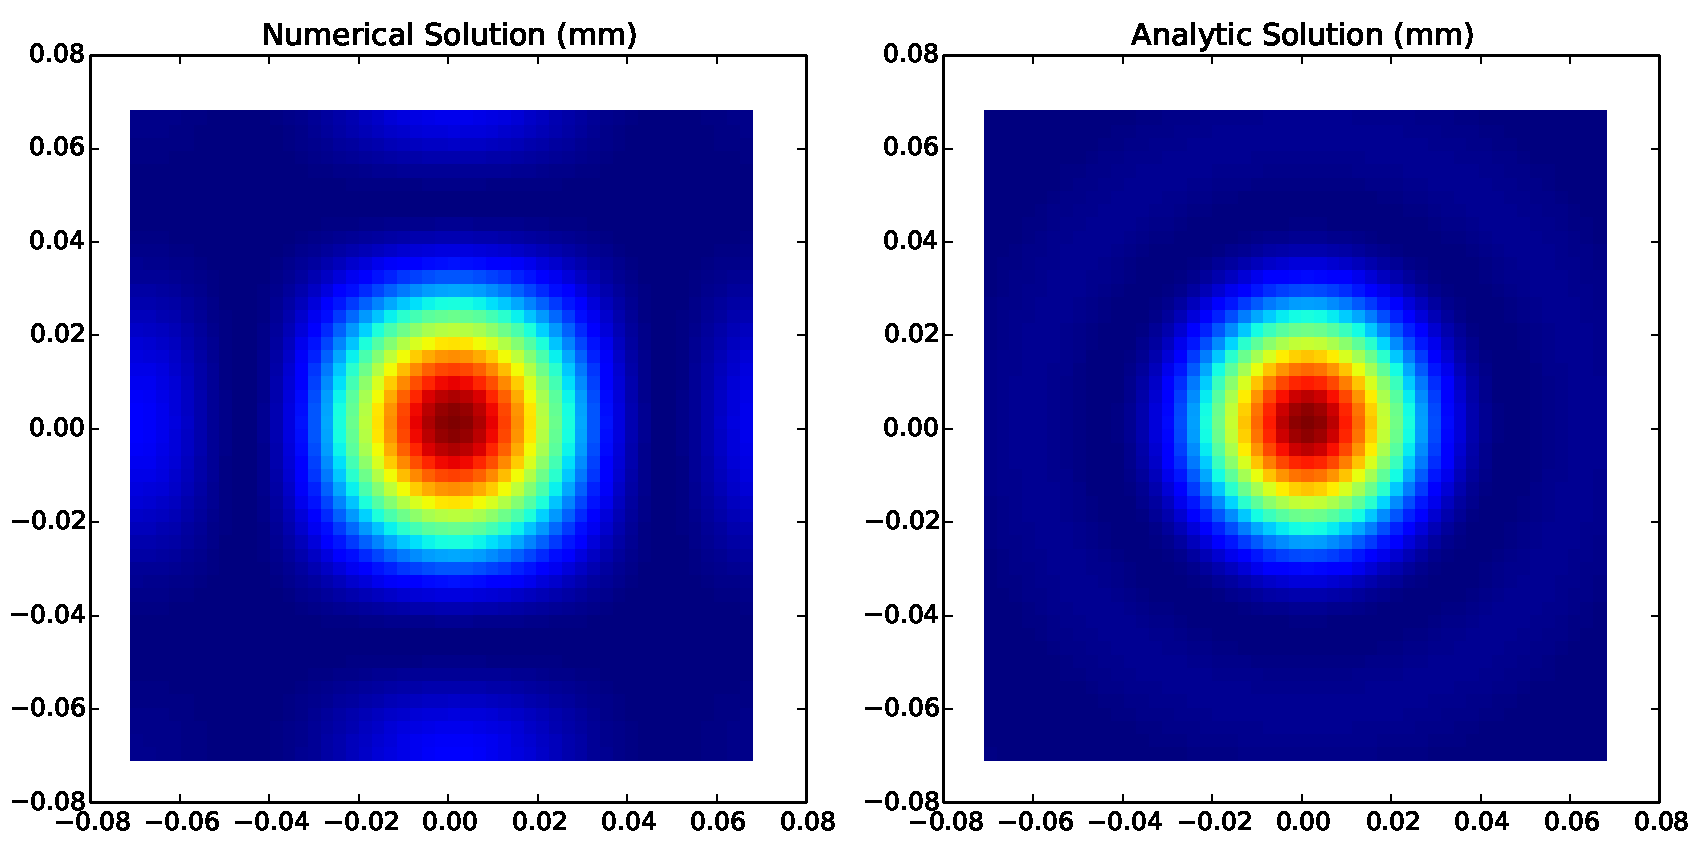
\includegraphics[width=1.0\textwidth]{figures/num_vs_an.pdf}
	\caption{Numerical solution and analytical solution for the intensity distribution}
	\label{fig:num_vs_an}
\end{figure}

\subsection{Image Size and Sampling}
The selection of the size of the imaging plane and sampling plane have a large effect on the numerical solution when found through the DFT.  The more highly sampled, the more similar the numeric solution will be to the analytical solution, however the computational resources put a limit on the number of samples. 

When moving to a sampled system, two things must be specified: (1) the size of the support structure (the total width over which the system will be sampled) and (2) the sample frequency or spacing.  The general sampling scenario is shown in Figure \ref{fig:GenSample}.  

\begin{figure}[H]
	\centering
		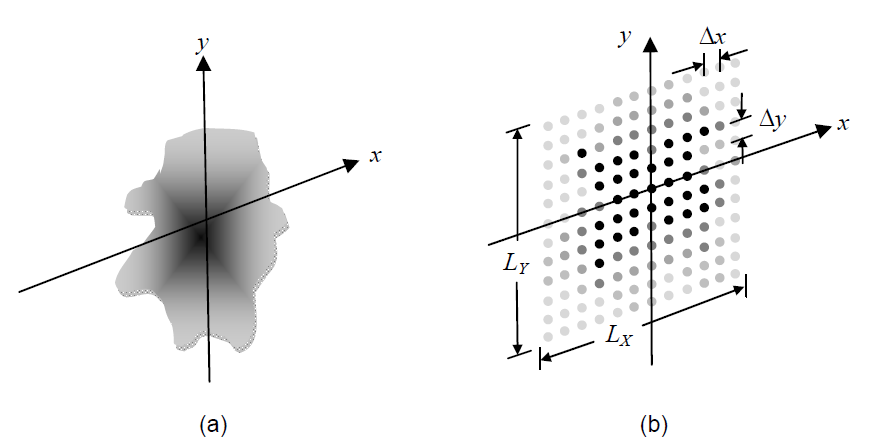
\includegraphics[width=0.8\textwidth]{figures/GeneralSampling.PNG}
	\caption{General two dimensional function: (a) analytic and (b) sampled \cite{CFO}.}
	\label{fig:GenSample}
\end{figure}

The side lengths (L$_x$ and L$_y$ in Figure \ref{fig:GenSample}) should be large enough to contain the entire significant portion of the original function, without taking up more memory than required.  Further the sample spacing ($\Delta$x and $\Delta$y) should be small enough to measure all of the features of the original function, however not so small to require the number of samples to be unreasonable.  

The limit on the maximum size of the sample spacing for a bandlimited signal is defined by the Shannon-Nyquist sampling theorem \cite{CFO}, given in Equation \ref{ShannonNyquist} below.  

\begin{equation}
\Delta x < \frac{1}{2B_x}  ,  \Delta y < \frac{1}{2B_y}
\label{ShannonNyquist}
\end{equation}

If the Shannon-Nyquist criterion is not met, the signal is said to be undersampled.  This leads to aliasing, where elements of the signal with high frequencies are mis-interpreted as low-frequency elements \cite{CFO}.  Figure \ref{fig:Aliasing} shows a signal (solid black line) that has been undersampled (grey 'x' markers) resulting in the appearance of a low frequency signal (dashed grey line).  

\begin{figure}[H]
	\centering
		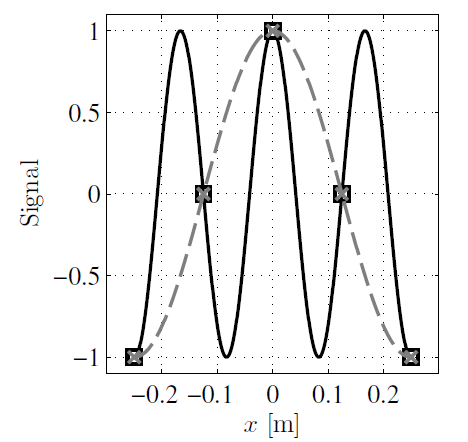
\includegraphics[width=0.6\textwidth]{figures/Alias.PNG}
	\caption{Aliasing of a high frequency signal through undersampling \cite{NSOWP}.}
	\label{fig:Aliasing}
\end{figure}

If the sampling rate is known, it is also possible to determine the maximum frequency that can be accurately represented by the samples.  This is called the Nyquist frequency, and is given by Equation \ref{Nyquist}.  

\begin{equation}
f_{NX} = \frac{1}{2\Delta x}  ,  f_{NY} = \frac{1}{2\Delta y} 
\label{Nyquist}
\end{equation}

Since real signals are not bandlimited, effective bandwidths can be calculated such that the significant frequencies are preserved and the amount of ripple generated by the cut-off of frequencies is tolerable.  According to \cite{CFO}, the effective bandwidth is found when the spectral power is 98\% of the total power in the spectrum.  This can be calculated using the method in \cite{CFO} using Parseval's theorem.  For example, the effective bandwidth for a circular function is given in Equation \ref{CircB}\cite{CFO}. 

\begin{equation}
for circ\left( \frac{\sqrt{x^2 + y^2}}{w}\right) ,  B_{eff} = \frac{5}{w} 
\label{CircB}
\end{equation}

Combining Equation \ref{CircB} with Equation \ref{ShannonNyquist} indicates that 10 samples across the radius of the circle is sufficient to encompass 98\% of the spectral power.  

In addition to aliasing, discretization results in "rippling and smearing in the spatial-frequency domain" and "virtual periodic replication in the spatial domain" \cite{NSOWP}. The stages of the discrete fourier transform are shown graphically in Figure \ref{fig:DFTGraphs} from \cite{NSOWP}.  

\begin{figure}[H]
	\centering
		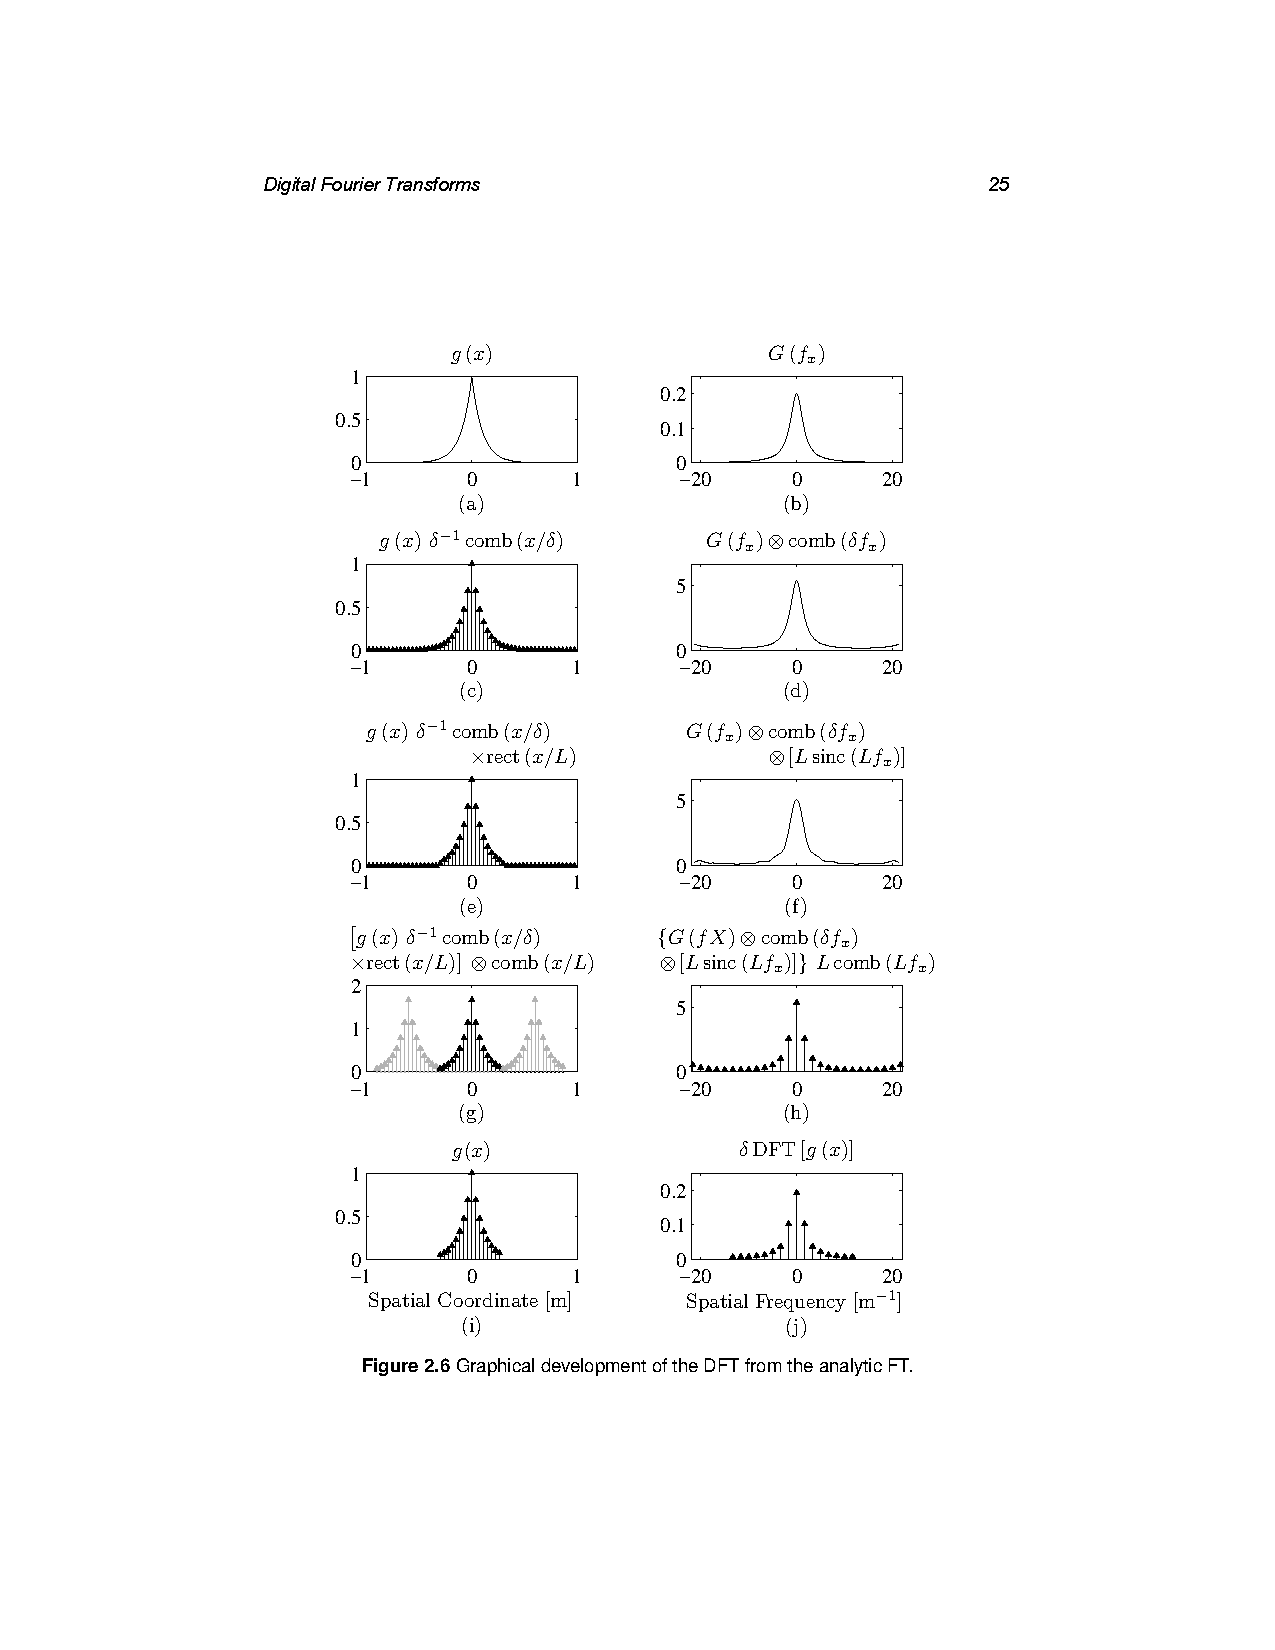
\includegraphics[trim=2cm 4cm 2cm 4cm, clip=true, width=0.8\textwidth]{figures/DFTGraphically.pdf}
	\caption{Steps of discrete fourier transform shown graphically \cite{NSOWP}.}
	\label{fig:DFTGraphs}
\end{figure}

Figure \ref{fig:DFTGraphs} shows pairs of images, where the left images are in the spatial domain ($g(x)$) and the right images are in the frequency domain ($G(f_x)$).  The first two images show the original function and its continuous fourier transform.  The second two images account for sampling with a spacing $\delta$.  Image (d) shows the first artifact of the discretization process in the 'lifting' of the ends of the function.  This is due to the periodic replication in the frequency domain.  The third set of images limits the functions to a finite image size ($L$), and in image (f) the rippling and smearing distortions are clear.  The fourth set of images show the sampling of the function in the frequency domain, with the result of virtual periodic  replication in the spatial domain shown in image (g).  Finally, image (i) shows the actual input function (with its limited spatial coordinate) and image (j) shows the sampled, band-limited DFT output. More information on the generation of this series of images and the distortions demonstrated can be found in \cite{NSOWP}. 

The discretization effects can be mitigated by proper sampling. To reduce rippling, the support width ($L_x$ and $L_y$) should be increased \cite{NSOWP}.  Similarly, to reduce aliasing, the sample spacing should be decreased (ie. the number of samples should be increased).  However, this returns to the original problem of limited computational resources.  The two requirements must be balanced based on the needs of the system.  




